\documentclass[convert={ghostscript,gsdevice=tiffg4,
outext=.tiff,density=1200}]{standalone}
    \usepackage{tikz}
    \usepackage{pgfplots}
    \usetikzlibrary{patterns}
\mathversion{bold}
\begin{document}
\Large
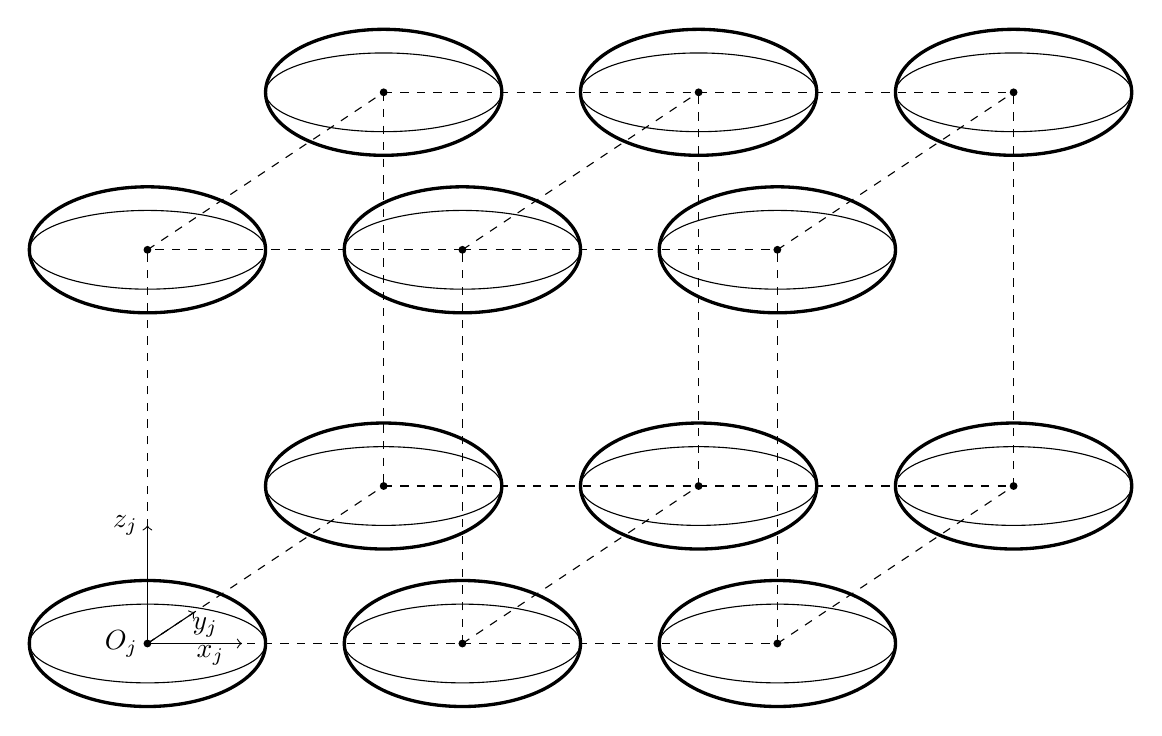
\begin{tikzpicture}%[scale=1.5]
\draw[->] (0,0) -- (0.6,0.4) node[anchor=north] {};
\draw[->] (0,0) -- (0,1.5) node[anchor=east] {$z_j$};
\draw[->] (0,0) -- (1.2,0) node[anchor=north] {};

\node[left] at (0,0) {$O_j$};
\node[right] at (0.45,0.2) {$y_j$};
\node[below] at (0.8,0.1) {$x_j$};

\draw[very thick] (0,0) ellipse (1.5 and 0.8);
\draw (0,0) ellipse (1.5 and .5);

\draw[very thick] (3,2) ellipse (1.5 and 0.8);
\draw (3,2) ellipse (1.5 and .5);

\draw[very thick] (0,5) ellipse (1.5 and 0.8);
\draw (0,5) ellipse (1.5 and .5);

\draw[very thick] (3,7) ellipse (1.5 and 0.8);
\draw (3,7) ellipse (1.5 and .5);


\draw[very thick] (4,0) ellipse (1.5 and 0.8);
\draw (4,0) ellipse (1.5 and .5);

\draw[very thick] (7,2) ellipse (1.5 and 0.8);
\draw (7,2) ellipse (1.5 and .5);

\draw[very thick] (4,5) ellipse (1.5 and 0.8);
\draw (4,5) ellipse (1.5 and .5);

\draw[very thick] (7,7) ellipse (1.5 and 0.8);
\draw (7,7) ellipse (1.5 and .5);

\draw[very thick] (8,0) ellipse (1.5 and 0.8);
\draw (8,0) ellipse (1.5 and .5);

\draw[very thick] (11,2) ellipse (1.5 and 0.8);
\draw (11,2) ellipse (1.5 and .5);

\draw[very thick] (8,5) ellipse (1.5 and 0.8);
\draw (8,5) ellipse (1.5 and .5);

\draw[very thick] (11,7) ellipse (1.5 and 0.8);
\draw (11,7) ellipse (1.5 and .5);

\draw[dashed] (0,0) -- (3,2);
\draw[dashed] (0,0) -- (0,5);
\draw[dashed] (3,7) -- (3,2);
\draw[dashed] (0,0) -- (4,0);
\draw[dashed] (0,5) -- (3,7);
\draw[dashed] (4,0) -- (4,5);
\draw[dashed] (4,5) -- (0,5);
\draw[dashed] (4,5) -- (7,7);
\draw[dashed] (4,0) -- (7,2);
\draw[dashed] (7,2) -- (7,7);
\draw[dashed] (3,2) -- (7,2);
\draw[dashed] (3,7) -- (7,7);
\draw[dashed] (4,0) -- (8,0);
\draw[dashed] (4,5) -- (8,5);
\draw[dashed] (7,7) -- (11,7);
\draw[dashed] (7,2) -- (11,2);
\draw[dashed] (8,0) -- (8,5);
\draw[dashed] (11,2) -- (11,7);
\draw[dashed] (8,0) -- (11,2);
\draw[dashed] (8,5) -- (11,7);


\node[circle, fill=black, inner sep=1pt] at (0,0) {};
\node[circle, fill=black, inner sep=1pt] at (3,2) {};
\node[circle, fill=black, inner sep=1pt] at (0,5) {};
\node[circle, fill=black, inner sep=1pt] at (3,7) {};

\node[circle, fill=black, inner sep=1pt] at (4,0) {};
\node[circle, fill=black, inner sep=1pt] at (7,2) {};
\node[circle, fill=black, inner sep=1pt] at (4,5) {};
\node[circle, fill=black, inner sep=1pt] at (7,7) {};

\node[circle, fill=black, inner sep=1pt] at (8,0) {};
\node[circle, fill=black, inner sep=1pt] at (11,2) {};
\node[circle, fill=black, inner sep=1pt] at (8,5) {};
\node[circle, fill=black, inner sep=1pt] at (11,7) {};

\end{tikzpicture}
\end{document}

%%% Local Variables: 
%%% mode: latex
%%% TeX-master: t
%%% End: 
